\documentclass{beamer}
\usepackage{amsmath}
\usepackage{amsfonts}
\usepackage{amssymb}
\usepackage{tikz}
\usepackage{multicol}
\usepackage[spanish]{babel}
\usepackage{pgfgantt}
\usepackage{xcolor}
%\usetheme{antibes}
%\usetheme[left,width=3cm]{goettingen}
%\usetheme{boadilla}
\usetheme{Warsaw}
\usetikzlibrary{arrows,positioning} 
\title[Coordinaci\'on Acad\'emica ]{Plan Org\'anico de la Coordinaci\'on Acad\'emica  }
\institute{ColombiaCrece}
\author{Sebasti\'an Rosales Cote}
\AtBeginSection[]
{
  \begin{frame}
    \frametitle{Tabla de contenidos}
  \begin{multicols}{2}
      \tableofcontents[currentsection]
    \end{multicols}
  \end{frame}
}
\begin{document}
\begin{frame}
\maketitle
\end{frame}
\begin{frame}
  \frametitle{Tabla de contenidos}
  \begin{multicols}{2}
      \tableofcontents
    \end{multicols}
\end{frame}
\section{Estructura}
\begin{frame}
\frametitle{El equipo}
\begin{tikzpicture}
\node[circle, draw=black, fill=blue!60](Dir) at (0,1.3) {Pame}; 
\node[circle, draw=black, fill=blue!40](Coor) at (0,0) {Sebas};
	\draw[<->]  (Dir) to (Coor);
\node[circle, draw=black, fill=blue!30](Natu) at (0,-2.5) {Bayron};
\node[circle, draw=black, fill=blue!30](Esp) at (-2.5,-0){Fede O};
	\draw[<->]  (Esp) to (Coor);
	\draw[<->]  (Natu) to (Coor);
\node[circle, draw=black, fill=blue!30](Mat) at (2.5, -0) {Aleja C};
	\draw[<->]  (Mat) to (Coor);
\node[circle, draw=black, fill=blue!30](Soc) at (-1.76, -1.76) {Andre R};
	\draw[<->]  (Soc) to (Coor);
\node[circle, draw=black, fill=blue!30](Ing) at (1.76, -1.76) {Cata E};
	\draw[<->]  (Ing) to (Coor);
\node[circle, draw=black, fill=blue!30](As1) at (2, 2) {Jose T};
\node[circle, draw=black, fill=blue!30](As2) at (-2, 2) {???};
	
	
\node (Mat1) at (3.5, 1.2){???};
	\draw [<->] (Mat) to( Mat1);
\node (Mat2) at (4, 0.4){Andre C};
	\draw [<->] (Mat) to( Mat2);
\node (Mat3) at (4, -0.4){Luis};
	\draw [<->] (Mat) to(Mat3);
\node (Mat4) at (3.5, -1.2){Oscar};
	\draw [<->] (Mat) to(Mat4);

\node (Esp1) at (-3.5, 1.2){???};
	\draw [<->] (Esp) to(Esp1);
\node (Esp2) at (-4, 0.4){???};
	\draw [<->] (Esp) to(Esp2);
\node (Esp3) at (-4, -0.4){Laura};
	\draw [<->] (Esp) to(Esp3);
\node (Esp4) at (-3.5, -1.2){Andre};
	\draw [<->] (Esp) to(Esp4);

\node (Soc1) at (-2.75, -2.9){Orduz};
	\draw [<->] (Soc1) to(Soc);
\node (Soc2) at (-3.15, -2.5){Lore};
	\draw [<->] (Soc2) to( Soc);
\node (Soc3) at (-3.5, -2){Qui\~nonez};
	\draw[<->] (Soc3) to (Soc);
\node (Soc4) at (-1.75, -3.1){Dani};
	\draw[<->] (Soc4) to (Soc);
	
\node (Ing1) at (2.75, -2.9){Andre G};
	\draw [<->] (Ing1) to(Ing);
\node (Ing2) at (3.15, -2.5){Angela};
	\draw [<->] (Ing2) to(Ing);
\node (Ing3) at (3.5, -2){Aleja C};
	\draw[<->] (Ing3) to (Ing);
\node (Ing4) at (1.75, -3.1){Diana};
	\draw[<->] (Ing4) to (Ing);

\node(Nat1) at (0,-4) {???};
	\draw [<->] (Nat1) to (Natu);
\node(Nat2) at (0.5,-3.75) {???};
	\draw [<->] (Nat2) to (Natu);
\node(Nat3) at (-0.5,-3.75) {???};
	\draw [<->] (Nat3) to (Natu);
\end{tikzpicture}
\end{frame}
\section{Descripci\'on General}
\begin{frame}
\begin{block}{Funciones de la coordinaci\'on}
La coordinaci\'on ac\'ademica planear\'a, ejecutar\'a y evaluar\'a los procesos ped\'agogicos que involucran los actores educativos  de ColombiaCrece. 
\end{block}
\end{frame}
\begin{frame}
\begin{center}
\begin{tikzpicture}
  \node[ circle,draw=black!50,fill=blue!40 ] (pl) at (3.5 ,-2.3){ Planeaci\'on  };
  \node[circle,draw=black!50,fill=blue!40] (ej) at (-3.5 ,-2.3 ){ Ejecuci\'on };
  \node[circle,draw=black!50,fill=blue!40] (ev) at (0,3.2 ){Evaluaci\'on };
     \draw[->] (pl) to [out=210,in=330](ej);
     \draw[->] (ej) to [out=90,in=210](ev);
     \draw[->] (ev) to [out=330,in=90](pl);
  \node[rectangle,draw=black!50,fill=orange] (pp) at (0,0 ){Actores Educativos  }; 
\end{tikzpicture}
\end{center}
\end{frame}
\begin{frame}
\begin{center}
\begin{tikzpicture}
  \node[ circle,draw=black!50,fill=blue!40 ] (pl) at (3.5 ,-2.3){ Planeaci\'on  };
  \node[circle,draw=black!50,fill=blue!40] (ej) at (-3.5 ,-2.3 ){ Ejecuci\'on };
  \node[circle,draw=black!50,fill=blue!40] (ev) at (0,3.2 ){Evaluaci\'on };
     \draw[->] (pl) to [out=210,in=330](ej);
     \draw[->] (ej) to [out=90,in=210](ev);
     \draw[->] (ev) to [out=330,in=90](pl);
  \node[rectangle,draw=black!50,fill=orange!25!green] (c) at (2,0 ){Curriculum };
   \node[rectangle,draw=black!50,fill=orange!25!blue] (d) at (-2,0 ){Docentes };
  \node[rectangle,draw=black!50,fill=orange!25!red] (r) at (0,1.5 ){Recursos };
  \node[rectangle,draw=black!50,fill=orange!25!yellow] (s) at (0,-1.5 ){Estudiantes };
   	 \draw[<->] (r) to [out=270,in=90](s);
     \draw[<->] (d) to [out=0,in=180](c);
     \draw[<->] (c) to (r);
     \draw[<->] (r) to (d);
     \draw[<->] (d) to (s);
     \draw[<->] (s) to (c);
 
\end{tikzpicture}
\end{center}
\end{frame}
\section{Curriculum}

\subsection{Estructura Curricular}
\begin{frame}
\begin{center}
\begin{tikzpicture}
	\filldraw[draw=black, fill=orange!25!green!25] (0,0) circle (3.5);
	 \node[rectangle,draw=black,fill=green] (mc) at (3,3 ){Marco Fil\'osofico};
  \node[rectangle,draw=black,fill=green] (ml) at (-3,3){Marco Legislativo};
  \node[rectangle,draw=black,fill=green] (mr) at (3,-3 ){Marco Referencial };
   \node[rectangle,draw=black,fill=green] (mp) at (-3,-3){Marco Pedag\'ogico};
   
  \node[rectangle,draw=black!50,fill=orange!25!green] (c) at (2,0 ){Objetivos };
  \node[rectangle,draw=black!50,fill=orange!25!green] (d) at (-2,0 ){Contenidos };
  \node[rectangle,draw=black!50,fill=orange!25!green] (r) at (0,1.5 ){M\'etodos };
   \node[rectangle,draw=black!50,fill=orange!25!green] (s) at (0,-1.5 ){Sistema de  Evaluaci\'on};
   \draw[<->] (r) to [out=270,in=90](s);
     \draw[<->] (d) to [out=0,in=180](c);
     \draw[<->] (c) to (r);
      \draw[<->] (r) to (d);
      \draw[<->] (d) to (s);
      \draw[<->] (s) to (c);
\end{tikzpicture}
\end{center}
\end{frame}
\subsection{Planeaci\'on}
\begin{frame}
\frametitle{Marco Legislativo}
\begin{tikzpicture}

\filldraw[draw=black, fill=orange!25!green!75] (0,0) -- (-6,-6)--(6,-6)--	 cycle;
\filldraw[draw=black, fill=orange!25!green!45] (0,0) -- (-4,-4)--(4,-4)--	 cycle;
\filldraw[draw=black, fill=orange!25!green!5](0,0) -- (-2,-2)--(2,-2)--	 cycle;
\node at (0,-5.25) {Decretos Distritales};
\node at (0,-4.75) {Leyes Distritales};
\node at (0,-3.25) {Decretos Nacionales};
\node at (0,-2.75) {Leyes Nacionales};
\node at (0,-0.95) {Art\'iculos};
\node at (0,-1.45) {Constitucionales};

\end{tikzpicture}
\end{frame}
\begin{frame}
\frametitle{Art\'iculos Constitucionales}
\textbf{Art. 26: }Toda persona es libre de escoger profesión u oficio.  \\
\textbf{Art. 27: }El Estado garantiza las libertades de ense\~nanza, aprendizaje, investigación y c\'atedra. \\
\textbf{Art 41:} En todas las instituciones de educaci\'on, oficiales o privadas, ser''an obligatorios el estudio de la Constituci\'on y la Instrucci\'on C\'ivica. As\'i mismo se fomentar\'an pr\'acticas democr\'aticas para el aprendizaje de los principios y valores de la participaci\'pn ciudadana. 
\end{frame}

\begin{frame}
\frametitle{Art\'iculo 67 I}
\begin{itemize}
\item La educaci\'on es un derecho de la persona y un servicio p\'ublico que tiene una funci\'on social; con ella se busca el acceso al conocimiento, a la ciencia, a la t\'ecnica, y a los dem\'as bienes y valores de la cultura.
\end{itemize}

\end{frame}

\begin{frame}
\frametitle{Art\'iculo 67 II}
\begin{itemize}
\item La educaci\'on formar\'a  al colombiano en el respeto a los derechos humanos, a la paz y a la democracia; y en la pr\'actica del trabajo y la recreaci\'on, para el mejoramiento cultural, cient\'ifico, tecnol\'ogico y para la protecci\'on del ambiente.
\end{itemize}
\end{frame}

\begin{frame}
\frametitle{Art\'iculo 67 III}
\begin{itemize}
\item El Estado, la sociedad y la familia son responsables de la educaci\'on, que ser\'a obligatoria entre los cinco y los quince años de edad y que comprender\'a como m\'inimo, un a\~no de preescolar y nueve de educación b\'asica.
\end{itemize}
\end{frame}

\begin{frame}
\frametitle{Art\'iculo 67 IV}
\begin{itemize}
\item La educaci\'on ser\'a gratuita en las instituciones del Estado, sin perjuicio del cobro de derechos académicos a quienes puedan sufragarlos.
\end{itemize}
\end{frame}
\begin{frame}
\frametitle{Art\'iculo 67 V}
\begin{itemize}
\item Corresponde al Estado regular y ejercer la suprema inspección y vigilancia de la educaci\'on con el fin de velar por su calidad, por el cumplimiento de sus fines y por la mejor formaci\'on moral, intelectual y f\'isica de los educandos; garantizar el adecuado cubrimiento del servicio y asegurar a los menores las condiciones necesarias para su acceso y permanencia en el sistema educativo. 
\end{itemize}
\end{frame}

\begin{frame}
\frametitle{Art\'iculo 67 VI}
\begin{itemize}
\item La Naci\'on y las entidades territoriales participar\'an en la direcci\'on, financiaci\'on y administraci\'on de los servicios educativos estatales, en los t\'erminos que se\~nalen la Constituci\'on y la ley. 
\end{itemize}
\end{frame}

\begin{frame}
\frametitle{Art\'iculo 3 Const. EE.UU. Mexicanos}
 Todo individuo tiene derecho a recibir educaci\'on. El Estado –Federaci\'on, Estados, Distrito Federal y Municipios–, impartir\'a educaci\'on preescolar, primaria, secundaria y media superior. La educación preescolar, primaria y secundaria conforman la educaci\'on b\'asica; \'esta y la media superior serán obligatorias.\\
 La educaci\'on que imparta el Estado tenderá a desarrollar arm\'onicamente, todas las facultades del ser humano y fomentar\'a en \'el, a la vez, el amor a la Patria, el respeto a los derechos humanos y la conciencia de la solidaridad internacional, en la independencia y en la justicia.
\end{frame}

\begin{frame}
\frametitle{Art\'iculo 27 Const. Reino de Espa\~na}
Todos tienen el derecho a la educaci\'on. Se reconoce la libertad de enseñ\~nanza. \\
La educaci\'on tendr\'a por objeto el pleno desarrollo de la personalidad humana en el respeto a los principios democr\'aticos de convivencia y a los derechos y libertades
fundamentales.\\
Los poderes p\'ublicos garantizan el derecho que asiste a los padres para que sus hijos reciban la formación religiosa y moral que est\'e de acuerdo con sus propias convicciones.\\
La ense\~nanza b\'asica es obligatoria y gratuita. 
\end{frame}
\begin{frame}
\frametitle{Art\'iculos 98-111 Const. Rep. Bolivariana de Venezuela}
La educaci\'on es un derecho humano y un deber social fundamental, es democr\'atica, gratuita y obligatoria.
El Estado la asumir\'a como funci\'on indeclinable y de m\'aximo inter\'es en todos sus niveles y modalidades, y como instrumento del conocimiento cient\'ifico, human\'istico y tecnol\'ogico [...]La educaci\'on es un servicio p\'ublico y est\'a fundamentada en erespeto a todas las corrientes del pensamiento, con la finalidad de desarrollar
el potencial creativo de cada ser humano[...]
\end{frame}
\begin{frame}
\frametitle{Art\'iculo 68 I}\begin{itemize}
\item Los particulares podr\'an fundar establecimientos educativos. La ley establecer\'a las condiciones para su creaci\'on y gesti\'on.\\
\item La comunidad educativa participar\'a en la direcci\'on de las instituciones de educaci\'on.\\
\item La enseñanza estar\'a a cargo de personas de reconocida idoneidad \'etica y pedag\'ogica. La Ley garantiza la profesionalizaci\'on y dignificaci\'on de la actividad docente. 
\end{itemize}
\end{frame}

\begin{frame}
\frametitle{Art\'iculo 68 II}
\begin{itemize}
\item Los padres de familia tendr\'an derecho de escoger el tipo de educaci\'on para sus hijos menores. En los establecimientos del Estado ninguna persona podr\'a ser obligada a recibir educaci\'on religiosa.\\
\item Las (sic) integrantes de los grupos \'etnicos tendr\'an derecho a una formaci\'on que respete y desarrolle su identidad cultural.\\
\item La erradicación del analfabetismo y la educaci\'on de personas con limitaciones f\'isicas o mentales, o con capacidades excepcionales, son obligaciones especiales del Estado. 
\end{itemize}
\end{frame}
\begin{frame}
\frametitle{Ley general de Educaci\'on(L115-1994)}

\textbf{Por tipo}

\begin{tikzpicture}
\node[rectangle,draw=black!50,fill=orange!25!blue] (pe) at (0,4 ){Educaci\'on };
  \node[rectangle,draw=black!50,fill=orange!25!blue!50] (ps) at (0,3 ){Formal};
    \draw[->] (pe) to (ps);
 \node[rectangle,draw=black!50,fill=orange!25!blue!50] (pi) at (4,3){No Formal };
    \draw[->] (pe) to (pi);
   \node[rectangle,draw=black!50,fill=orange!25!blue!50] (pn) at (-4,3 ){Informal  };
    \draw[->] (pe) to (pn);
\end{tikzpicture}
\end{frame}
\begin{frame}
\frametitle{Ley general de Educaci\'on(L115-1994)}

\textbf{Por poblaci\'on }

\begin{tikzpicture}
\node[rectangle,draw=black!50,fill=orange!25!blue] (pe) at (0,4 ){Educaci\'on };
  \node[rectangle,draw=black!50,fill=orange!25!blue!50] (ps) at (0,3 ){Edad Escolar};
    \draw[->] (pe) to (ps);
     \node[rectangle,draw=black!50,fill=orange!25!blue!50] (ps) at (0,1 ){Cap. Especiales, Rehab. Social};
    \draw[->] (pe) to (ps);
 \node[rectangle,draw=black!50,fill=orange!25!blue!50] (pi) at (5,3){Adultos};
    \draw[->] (pe) to (pi);
   \node[rectangle,draw=black!50,fill=orange!25!blue!50] (pn) at (-5,3 ){Campesinos};
    \draw[->] (pe) to (pn);
      \node[rectangle,draw=black!50,fill=orange!25!blue!50] (ps) at (2.5,2 ){Gr. \'Etnicos};
    \draw[->] (pe) to (ps);
 \node[rectangle,draw=black!50,fill=orange!25!blue!50] (pi) at (-2.5,2){Limitaciones};
    \draw[->] (pe) to (pi);

\end{tikzpicture}
\end{frame}
\begin{frame}
\frametitle{Ley general de Educaci\'on(L115-1994)}
\begin{block}
{Prestaci\'on del servicio educativo}
" El servicio educativo ser\'a prestado en las instituciones educativas del Estado. Igualmente los particulares podr\'an fundar establecimientos educativos en las condiciones que para su creaci\'on y gestión establezcan las normas pertinentes y la reglamentación del Gobierno Nacional.\\
De la misma manera el servicio educativo podr\'a prestarse en instituciones educativas de car\'acter comunitario, solidario, cooperativo o sin \'animo de lucro."
\end{block}
\end{frame}


 
\begin{frame}
\frametitle{Ley general de Educaci\'on(L115-1994)}
\begin{block}{Fines de la Educaci\'on}
\begin{enumerate}
\item Dllo. personalidad.
\item Respeto a los DD.HH.
\item Participaci\'on Pol\'itica.
\item Respeto a la Ley.
\item Adquisic\'on de Conocimientos
\end{enumerate}
\end{block}
\end{frame}
\begin{frame}
\frametitle{Ley general de Educaci\'on(L115-1994)}
\begin{block}{Fines de la Educaci\'on}
\begin{enumerate}
\item Comprensi\'on Cr\'itica de la cultura y la diversidad.
\item Conciencia de la soberania nacional. 
\item Dllo de la capacidad cr\'itica, reflexica y an\'alitica.
\item Conciencia   de la conservaci\'on, protecci \'on y mejoramiento del Medio Ambiente. 
\item Formaci\'on para el trabajo 
\item Salud
\item Desarrollo Tecnol\'ogico

\end{enumerate}
\end{block}
\end{frame}
\begin{frame}
\frametitle{Ley general de Educaci\'on(L115-1994)}
\begin{block}{Educaci\'on Formal.}
" Se entiende por educaci\'on formal aquella que se imparte en establecimientos educativos aprobados, en una secuencia regular de ciclos lectivos, con sujeción a pautas
curriculares progresivas, y conducente a grados y t\'itulos. "
\\ Tres niveles: \begin{enumerate}
\item Un grado-Preescolar
\item  Cinco de B\'asica primaria y Cuatro de B\'asica Secundaria
\item  Dos de Media
\end{enumerate}
\end{block}
\end{frame}

\begin{frame}
\frametitle{Ley general de Educaci\'on(L115-1994)}
\begin{block}{Educaci\'on Formal.Ense\~naza obligatoria}
 \begin{enumerate}
\item Constituci\'on *  \checkmark
\item  Educaci\'on F\'isica *
\item  Medio ambiente \checkmark
\item Formaci\'on en Valores Humanos \checkmark
\item  Educaci\'on Sexual
\end{enumerate}
\end{block}
\end{frame}

\begin{frame}
\frametitle{Ley general de Educaci\'on(L115-1994)}
\begin{block}{Educaci\'on Formal. Areas(sic) Obligatorias y Fundamentales (80\% del plan de estudios }
 \begin{enumerate}
\item Naturale
\item  Sociales (Sin Filosof\'ia)
\item  Art\'istica
\item \'Etica y Valores
\item  Educaci\'on F\'isica, Recreaci\'on y Deportes
\item Matem\'aticas
\item Tecnolog\'ia e Inform\'atica.  
\end{enumerate}
\end{block}
\end{frame}
\begin{frame}
\frametitle{Ley general de Educaci\'on(L115-1994)}
\begin{block}{Educaci\'on Formal. Religiosa}
La educaci\'on religiosa se ofrecer\'a en todos los establecimientos educativos, observando la garant\'ia constitucional seg\'un la cual, en los establecimientos del Estado ninguna persona podr\'a ser obligada a
recibirla. 
\end{block}
\end{frame}

\begin{frame}
\frametitle{Ley general de Educaci\'on(L115-1994)}
\begin{block}{Educaci\'on No Formal. Definici\'on}
" La educaci\'on no formal es la que se ofrece con el objeto de complementar, actualizar, suplir conocimientos y formar en aspectos acad\'emicos o laborales sin sujeci\'on al sistema de niveles y grados establecidos en el art\'iculo 11 de esta Ley. \newline
[...]\\
En  las instituciones de educaci\'on no formal se podr\'an ofrecer
programas de formaci\'on laboral en artes y oficios, de formaci\'on acad\'amica y en materias conducentes a la validaci\'on de niveles y grados propios de la educaci\'on formal, definidos en la presente Ley "
\end{block}
\end{frame}
\begin{frame}
\begin{block}{Educaci\'on Informal. Definici\'on}
Se considera educaci\'on informal todo conocimiento libre y espont\'aneamente adquirido, proveniente de personas, entidades, medios masivos de comunicaci\'on, medios
impresos, tradiciones, costumbres, comportamientos sociales y otros no estructurados.
\end{block}
\end{frame}
\begin{frame}
\frametitle{Ley general de Educaci\'on(L115-1994)}
\begin{block}{Educaci\'on para Adultos. Objetivos}
 \begin{enumerate}
\item Adquirir y actualizar su formaci\'on b\'asica y facilitar el acceso a los distintos niveles educativos; 
\item  Erradicar el analfabetismo
\item  Actualizar los conocimientos, seg\'un el nivel de educaci\'on,
\item Desarrollar la capacidad de participaci\'on en la vida econ\'omica, pol\'itica, social, cultural y comunitaria.
\end{enumerate}
\end{block}
\end{frame}
\begin{frame}
\frametitle{Ley general de Educaci\'on(L115-1994)}
\begin{block}{Educaci\'on para Adultos. Validaci\'on }
El Estado ofrecer\'a a los adultos la posibilidad de validar la educaci\'on b\'asica o media y facilitar\'a su ingreso a la educaci\'on superior, de acuerdo con los requisitos establecidos en la Ley.\\
Las instituciones educativas autorizadas podr\'an reconocer y validar los conocimientos, experiencias y pr\'acticas de los adultos, sin la exigencia de haber cursado determinado grado de escolaridad formal, o los programas de educación no formal del arte u oficio de que se trate, cumpliendo los requisitos que para tal fin establezca el Gobierno Nacional, y con sujeci\'on a la Ley 30 de 1992, o las normas que la modifiquen, adicionen o sustituya
\end{block}
\end{frame}
\begin{frame}
\frametitle{Ley general de Educaci\'on(L115-1994)}
\begin{block}{Proyecto Educativo Institucional }
[...] en el que se especifiquen entre otros aspectos, los principios y fines del establecimiento, los recursos docentes y did\'acticos  disponibles y necesarios, la estrategia pedag\'ogica, el reglamento para docentes y estudiantes y el sistema de gesti\'on, todo ello encaminado a cumplir con las disposiciones de la presente ley y sus reglamentos. \newline
[...]
\newline
PARAGRAFO. El Proyecto Educativo Institucional debe responder a situaciones y necesidades de los educandos, de la comunidad local, de la regi\'on y del pa\'is, ser concreto, factible y evaluable.
\end{block}
\end{frame}

\begin{frame}
\frametitle{Ley general de Educaci\'on(L115-1994)}
\begin{block}{Curr\'iculo}
Es el conjunto de criterios, planes de estudio, programas, metodolog\'ias, y procesos que contribuyen a la formaci\'on integral y a la construcci\'on de la identidad cultural nacional, regional y local, incluyendo tambi\'en los recursos humanos, acad\'emicos y f\'isicos para poner en pr\'actica las pol\'iticas y llevar a cabo el proyecto educativo institucional.
\end{block}
\end{frame}

\begin{frame}
\frametitle{Ley general de Educaci\'on(L115-1994)}
\begin{block}{Evaluaci\'on}
\begin{enumerate}
\item Evaluaci\'on docente (c/6 yr) Institucional
\item Evaluaci\'on a Directivos (Secretaria)
\item Evaluaci\'on Institucional Anual (MEN)
\end{enumerate}
\end{block}
\end{frame}

\begin{frame}
\frametitle{Ley general de Educaci\'on(L115-1994)}
\begin{block}{Organizaci\'on Administrativa del Servicio}
\begin{enumerate}
\item M\'inimo de horas Semanales (Formal)
\item Manual de convivencia
\item Formal: T\'itulos y Validaciones de los Grados.
\item No formal: " 	certificados de técnico en los programas de artes y oficios y de formación vocacional. "
\item Representante de Estudiantes. 
\item Personero de los Estuduantes, 
\item Formal: Seguro de Salud Obligatorio
\end{enumerate}
\end{block}
\end{frame}

\begin{frame}
\frametitle{Ley general de Educaci\'on(L115-1994)}
\begin{block}{Requisitos de los establecimientos educativos}
\begin{enumerate}
\item Licencia o reconocimiento de car\'acter oficial.
\item Estructura administrativa.
\item Planta f\'isica y medios educativos adecuados. (MEN) 
\item Proyecto Educativo Institucional. (MEN) 
\item Biblioteca,  infraestructura para art\'isticas y deportivas y \'organo de difusi\'on. 
\end{enumerate}
\end{block}
\end{frame}

\begin{frame}
\begin{block}{Plan de Estudios}
Es el esquema estructurado de las \'areas obligatorias y fundamentales y de \'areas optativas con sus respectivas asignaturas, que forman parte del curr\'iculo de los establecimientos educativos.\\
En la educaci\'on formal, dicho plan debe establecer los objetivos por niveles, grados y \'areas, la metodolog\'ia, la distribuci\'on del tiempo y los criterios de evaluaci\'on y administraci\'on, de acuerdo con el Proyecto Educativo Institucional y con las disposiciones legales vigentes.
\end{block}
\end{frame}

\begin{frame}
\frametitle{Plan Nacional de Desarrollo Educativo}
\end{frame}

\begin{frame}
\frametitle{Estandares  y Lineamientos Curriculares}
\begin{tikzpicture}
\node[rectangle,draw=black!50,fill=orange!25!blue] (pe) at (0,4 ){Art\'iculo 23. \'Areas Fundamentales y obligatorias  };
 \node[rectangle,draw=black!50,fill=orange!25!blue!50] (pi) at (3,3){Estandares };
    \draw[->] (pe) to (pi);
   \node[rectangle,draw=black!50,fill=orange!25!blue!50] (pn) at (-3,3 ){Lineamientos};
    \draw[->] (pe) to (pn);
    \draw[->] (pn) to (pi);
     \node[rectangle,draw=black!50,fill=orange!25!blue!50] (pa) at (3,2){Materializaci\'on de los lineamientos };
    \draw[->] (pi) to (pa);
   \node[rectangle,draw=black!50,fill=orange!25!blue!50] (pb) at (-3,2 ){ ... filosof\'ia de las \'areas. };
    \draw[->] (pn) to (pb);
\end{tikzpicture}
\end{frame}

\begin{frame}
\frametitle{D114-1996}
\end{frame}
\begin{frame}
\frametitle{Objetivos}
\begin{center}
\begin{tikzpicture}
  \node[rectangle,draw=black!50,fill=orange!25!green] (pe) at (0,4 ){Perfil del egresado };
  \node[rectangle,draw=black!50,fill=orange!25!green!50] (ps) at (0,2 ){Prop.  Sociales};
    \draw[->] (pe) to [out=270,in=90](ps);
  \node[rectangle,draw=black!50,fill=orange!25!green!50] (pm) at (-2.25,1 ){Prop. Mate. };
    \draw[->] (pe) to [out=270,in=90](pm);
   \node[rectangle,draw=black!50,fill=orange!25!green!50] (pes) at (2.25,1 ){Prop. Espa\~nol };
    \draw[->] (pe) to [out=270,in=90](pes);
   \node[rectangle,draw=black!50,fill=orange!25!green!50] (pi) at (4.,2 ){Prop. Ingl\'es };
    \draw[->] (pe) to [out=270,in=90](pi);
   \node[rectangle,draw=black!50,fill=orange!25!green!50] (pn) at (-4,2 ){Prop. Naturales  };
    \draw[->] (pe) to [out=270,in=90](pn);

\end{tikzpicture}
\end{center}
\end{frame}
\begin{frame}
\frametitle{De objetivos a contenidos}
\begin{center}
\begin{tikzpicture}
\node[rectangle,draw=black!50,fill=orange!25!green!50] (pe) at (0,4 ){Prop\'osito Sociales};
\node[rectangle,draw=black!50,fill=orange!25!green!25] (ps) at (0,2 ){Objetivo-Contenido};
    \draw[->] (pe) to [out=270,in=90](ps);
  \node[rectangle,draw=black!50,fill=orange!25!green!25] (pm) at (-2.25,1 ){Objetivo-Contenido };
    \draw[->] (pe) to [out=270,in=90](pm);
   \node[rectangle,draw=black!50,fill=orange!25!green!25] (pes) at (2.25,1 ){Objetivo-Contenido };
    \draw[->] (pe) to [out=270,in=90](pes);
   \node[rectangle,draw=black!50,fill=orange!25!green!25] (pi) at (4.,2 ){Objetivo-Contenido };
    \draw[->] (pe) to [out=270,in=90](pi);
   \node[rectangle,draw=black!50,fill=orange!25!green!25] (pn) at (-4,2 ){Objetivo-Contenido};
    \draw[->] (pe) to [out=270,in=90](pn);

\end{tikzpicture}
\end{center}
\end{frame}

\begin{frame}
\frametitle{Contenidos}
\begin{block}{Evaluaci\'on de Contenidos} 
\begin{enumerate}
\item \textbf{Validez:} El contenido es aut\'entico y verdadero.El contenido persigue  EL PROP\'OSITO.  
\item\textbf{Significatividad:} El contenido es profundo e importante para el estudiante.
\item \textbf{Inter\'es:} El contenido es interesante para el estudiantes (El criterio menos fuerte) 
\item \textbf{Aprendibilidad y Ense\~nabilidad: }El contenido puede ser ense\~ado por los profesores y aprendido por los estudiantes.
\end{enumerate}
\end{block}
\end{frame}

\begin{frame}
\frametitle{Contenidos}
\begin{block}{Criterios para selecci\'on de contenidos} 
\begin{enumerate}
\item Preferir los contenidos m\'as \textbf{pr\'oximos}  (Geogr\'afica y temporalmente, y por intereses)
\item Preferir los contenidos \textbf{prerrequisitos} de los ulteriores
\item Preferir lo contenidos con mayor \textbf{transferencia} (\'utiles en m\'as ambitos)
\item Preferir los contenidos m\'as \textbf{consolidados} (Con mayor evidencia y menos discutibles cientificamente)
\end{enumerate}
\end{block}
\end{frame}

\begin{frame}

\frametitle{Precisiones Terminol\'ogicas}
\begin{block}
{?`Cu\'al es la diferencia?}
\begin{itemize}
\item \textbf{Fin}
\item \textbf{Prop\'osito} 
\item \textbf{Meta} 
\item \textbf{Objetivo}
\end{itemize}
\end{block}
\end{frame}

\begin{frame}
\frametitle{Precisiones Terminol\'ogicas}
\begin{block}{?` Cu\'al es la diferencia? }
\begin{itemize}
\item \textbf{Fin:}\\ Intencionalidad no cuantificable y no planificable. Involucra  un sistema externo al planeado. 
\item \textbf{Prop\'osito:} \\Intencionalidad de un objetivo. 
\item \textbf{Meta:} \\Criterio umbral cuantificable y planificable que determina si el objetivo fue cumplido. 
\item \textbf{Objetivo}
\end{itemize}
\end{block}
\end{frame}


\begin{frame}
\frametitle{Precisiones Terminol\'ogicas}
\begin{block}{Ejemplo 1 }
\begin{itemize}
\item \textbf{Objetivo}: Bajar de peso.
\end{itemize}
\end{block}
\end{frame}
\begin{frame}
\frametitle{Precisiones Terminol\'ogicas}
\begin{block}{Ejemplo 1 }
\begin{itemize}
\item \textbf{Fin:} Satisfacer patrones de belleza f\'isica establecidos por la sociedad occidental .
\item \textbf{Prop\'osito:} Ligarme a Pepit@
\item \textbf{Meta:} Bajar 3 kilos en 15 dias. 
\end{itemize}
\end{block}
\end{frame}
\begin{frame}
\frametitle{Precisiones Terminol\'ogicas}
\begin{block}{Ejemplo 2 }
\begin{itemize}
\item \textbf{Objetivo}: Calcular sumas.
\end{itemize}
\end{block}
\end{frame}


\begin{frame}
\frametitle{Precisiones Terminol\'ogicas}
\begin{block}{Ejemplo 2 }
\begin{itemize}
\item \textbf{Fin:} Cumplir criterios de la sociedad materialista  que definen a un ser humano \'util como uno capaz de integrarse al sistema laboral.
\item \textbf{Prop\'osito:} Resolver problemas de la vida diaria 
\item \textbf{Meta:} Calculan 3 sumas de hasta 3 digitos y 2 decimales  en una hora. 
\end{itemize}
\end{block}
\end{frame}

\begin{frame}
\frametitle{Redacci\'on de objetivos}
\begin{center}
\begin{table}
\begin{tabular}{|c|c|}
\hline
\textbf{Forma}&\textbf{Fondo}\\
\hline
Criterios Smart modificados (SEAR) &Taxonom\'ia de Bloom \\
\hline
\end{tabular}
\end{table}
\end{center}
\end{frame}

\begin{frame}
\frametitle{Objetivos SMART, SEAR}
\begin{center}
\begin{table}
\begin{tabular}{|l|c|c|}
\hline
\textbf{Acr\'onimo}&\textbf{Significado}&\textbf{Modificaci\'on}\\
\hline
\textbf{S}pecific &Especifico & N/A \\
\textbf{M}easurable&Mesurable & Evaluable  \\
\textbf{A}chivable &Alcanzable & N/A \\
\textbf{R}ealistic &Realista & N/A \\
\textbf{T}imable &Acotado en el tiempo & Est\'a impl\'icito en \\
 &tiempo & la divisi\'on cronol\'ogica\\
\hline
\end{tabular}
\end{table}
\end{center}

\end{frame}

\begin{frame}
\frametitle{Taxonom\'ia de Bloom}
\begin{center}
\begin{tikzpicture}
\node[rectangle,draw=black!50,fill=orange!25!green!50] (a) at (0,0 ){Conocimiento};
\node[rectangle,draw=black!50,fill=orange!25!green!50] (b) at (3.5,0 ){Comprensi\'on};
\node[rectangle,draw=black!50,fill=orange!25!green!50] (c) at (7,0 ){Aplicaci\'on};
\node[rectangle,draw=black!50,fill=orange!25!green!50] (d) at (7,3 ){An\'alisis};
\node[rectangle,draw=black!50,fill=orange!25!green!50] (e) at (3.5,3 ){S\'intesis };
\node[rectangle,draw=black!50,fill=orange!25!green!50] (f) at (0,3){Evaluaci\'on};
    \draw[->] (a) to (b);
      \draw[->] (b) to (c);
        \draw[->] (c) to (d);
          \draw[->] (d) to (e);
            \draw[->] (e) to (f);
\node[rectangle,draw=black!50,fill=orange!25!green!25] (ab) at (0,-1 ){Memoria};
\node[rectangle,draw=black!50,fill=orange!25!green!25] (ac) at (3.5,-1 ){Incorporar};
\node[rectangle,draw=black!50,fill=orange!25!green!25] (ad) at (7,-1 ){Exteriorizar};
\node[rectangle,draw=black!50,fill=orange!25!green!25] (ae) at (7,2 ){Descomponer};
\node[rectangle,draw=black!50,fill=orange!25!green!25] (af) at (3.5,2 ){Recomponer, crear };
\node[rectangle,draw=black!50,fill=orange!25!green!25] (ag) at (0,2){Criticar, proponer};
 \draw[->] (a) to (ab);
      \draw[->] (b) to (ac);
        \draw[->] (c) to (ad);
          \draw[->] (d) to (ae);
            \draw[->] (e) to (af);
             \draw[->] (f) to (ag);
\end{tikzpicture}
\end{center}
\end{frame}
\begin{frame}
\begin{block}{Retroalimentaci\'on de los directores}
\begin{enumerate}
\item Reforzar la horizontalidad.
\item Integrar Pensamiento Integral
\item Integrar Alfabetizaci\'on 
\item Sociales: Ampliar mec\'anismos de Participaci\'on Ciudadana. 
\item Sociales: Incluir derecho-deber del voto. 
\end{enumerate}

\end{block}
\end{frame}
\begin{frame}
\frametitle{De objetivos a m\'etodo y evaluaci\'on}
\begin{center}
\begin{tikzpicture}
  \node[rectangle,draw=black!50,fill=orange!25!green!50] (m) at (-3,-2 ){M\'etodo Sociales};
  \node[rectangle,draw=black!50,fill=orange!25!green!50] (e) at (3,-2 ){Evaluaci\'on Sociales};
  \node[rectangle,draw=black!50,fill=orange!25!green!50] (pe) at (0,2 ){Prop\'osito Sociales};
 
      \draw[<->] (m) to (e);
      \draw[->] (pe) to (e);
      \draw[->] (pe) to (m);
\end{tikzpicture}
\end{center}
\end{frame}


\begin{frame}
\frametitle{Definici\'on evaluaci\'on}
\begin{center}
\textbf{Proceso} sist\'emico donde se emiten juicios de valor en relaci\'on a unos \textbf{objetivos preestablecidos}. (Alvarez Mendez)
\end{center}
\end{frame}
\begin{frame}
\frametitle{Preguntas de evaluaci\'on}
\begin{center}
\begin{tikzpicture}
  \node[rectangle,draw=black!50,fill=orange!25!green!50] (que) at (-1,0 ){?`Qu\'e?};
  \node[rectangle,draw=black!50,fill=orange!25!green!50] (para) at (-1,-1 ){?`Para qu\'e?};
  \node[rectangle,draw=black!50,fill=orange!25!green!50] (conque) at (-1,- 2){?`Con qu\'e?};
  \node[rectangle,draw=black!50,fill=orange!25!green!50] (pq) at (-1,-3){?`Por qu\'e?};
  \node[rectangle,draw=black!50,fill=orange!25!green!50] (quien) at (-1,-4 ){?`Qui\'en?}; 
  \node[rectangle,draw=black!50,fill=orange!25!green!50] (aquien) at (-1,-5){?`A qui\'en?};
  \node[rectangle,draw=black!50,fill=orange!25!green!50] (cuando) at (-1,-6 ){?`Cu\'ando?};
   \node[rectangle,draw=black!50,fill=orange!25!green!50] (objeto) at (3,0 ){Objeto de evaluaci\'on};
    \draw[->] (que) to (objeto);
     \node[rectangle,draw=black!50,fill=orange!25!green!50] (finalidad) at (3,-1 ){Finalidad};
    \draw[->] (para) to (finalidad);
     \node[rectangle,draw=black!50,fill=orange!25!green!50] (instr) at (3,-2 ){Instrumento};
    \draw[->] (conque) to (instr);
     \node[rectangle,draw=black!50,fill=orange!25!green!50] (corr) at (3,-3){Corregir y Revisar};
    \draw[->] (pq) to (corr);
     \node[rectangle,draw=black!50,fill=orange!25!green!50] (eval) at (3,-4){Evaluador};
    \draw[->] (quien) to (eval);
    \node[rectangle,draw=black!50,fill=orange!25!green!50] (desemp) at (3,-5 ){Desempe\~no};
    \draw[->] (aquien) to (desemp);
     \node[rectangle,draw=black!50,fill=orange!25!green!50] (momento) at (3,-6){Momento};
    \draw[->] (cuando) to (momento);
\end{tikzpicture}
\end{center}
\end{frame}
\begin{frame}

\frametitle{Precisiones Terminol\'ogicas}
\begin{block}
{?`Cu\'al es la diferencia?}
\begin{itemize}
\item \textbf{Evaluar}
\item \textbf{Calificar} 
\item \textbf{Acreditar} 
\item \textbf{Certificar}
\end{itemize}
\end{block}
\end{frame}

\begin{frame}
\frametitle{Precisiones Terminol\'ogicas}
\begin{block}{?` Cu\'al es la diferencia? }
\begin{itemize}
\item \textbf{Evaluar}: Proceso sist\'emico donde se emiten juicios de valor en relaci\'on a unos objetivos preestablecidos. (Proceso)
\item \textbf{Calificar} : Traducci\'on n\'umerica de una evaluaci\'on. (Evento)
\item \textbf{Acreditar} : Dar fe de un proceso. (Evento)
\item \textbf{Certificar}: Dar fe de un resultado. (Evento)
\end{itemize}
\end{block}
\end{frame}

\begin{frame}
\begin{block}{ ?` Para qu\'e?}
\begin{itemize}
\item Diagnostica 
\item Formativa
\item Sumativa
\end{itemize}
\end{block}
\end{frame}
\begin{frame}
\begin{block}{ ?` Qui\'en ?}
\begin{itemize}
\item Autoevaluaci\'on
\item Coevaluaci\'on
\item Heteroevaluaci\'on
\end{itemize}
\end{block}
\end{frame}
\begin{frame}
\begin{block}{ ?` Cu\'ando ?}
\begin{itemize}
\item Inicial
\item Procesual
\item Final
\item Diferida
\end{itemize}
\end{block}
\end{frame}
\begin{frame}
\frametitle{Precisiones terminol\'ogicas}
\begin{center}
\begin{tikzpicture}

\filldraw[draw=black, fill=orange!25!green!5] (0,0) circle (3);
\node at (0,2.5) {Metodolog\'ia};
\node at (-4.5,2.5) {C.Crece};
\filldraw[draw=black, fill=orange!25!green!25] (0,-0.5) circle (2.5);
\node at (0,1.5) {M\'etodo};
\node at (-4.5,1.5) {Materia};
\filldraw[draw=black, fill=orange!25!green!45] (0,-1) circle (2);
\node at (0,0.5) {Estrat\'egia};
\node at (-4.5,0.5) {Curso};
\filldraw[draw=black, fill=orange!25!green!65] (0,-1.5) circle (1.5);
\node at (0,-0.5) {T\'ecnica};
\node at (-4.5,-0.5) {Clase};
\filldraw[draw=black, fill=orange!25!green!75] (0,-2) circle (1);
\node at (0,-2) {Actividad};
\node at (-4.5,-2) {Actividad};
\end{tikzpicture}
\end{center}
\end{frame}
\begin{frame}
\frametitle{Diagrama de Gannt para la Planeaci\'on del Curriculum}
\fontsize{9pt}{10}\selectfont
\begin{center}

\begin{ganttchart}[
y unit title=0.4cm,
y unit chart=0.35cm,
x unit =0.75 cm,
vgrid,
time slot format=isodate,
compress calendar,
title/.append style={draw=none, fill=blue!50!black},
title label font=\sffamily\bfseries\color{white},
title label node/.append style={below=-1.6ex},
title left shift=.05,
title right shift=-.05,
title height=1,
bar/.append style={draw=none, fill=orange!50!green!50},
bar height=.6,
bar label font=\normalsize\color{black!50},
group right shift=0,
group top shift=.6,
group height=.3,
group peaks height=.2,
bar incomplete/.append style={fill=orange}
]{2014-08-01}{2015-06-30}

\gantttitlecalendar{year,month=shortname} \\



\ganttset{progress label text={}, link/.style={black, -to}}
\ganttgroup{Cont.-Objetivos}{2014-08-01}{2015-01-31} \\
\ganttbar[progress=100, bar progress label font=\small\color{orange!25!green!50!black},
bar progress label node/.append style={right=4pt},
bar label font=\normalsize\color{orange!25!green!50!black},name=R]{Planeaci\'on }{2014-08-01}{2014-11-15} \\
\ganttbar[progress=0,name=T]{Ejecuci\'on}{2014-11-01}{2014-12-20} \\
\ganttbar[progress=0,name=E]{Evaluaci\'on}{2014-12-01}{2015-01-31} \\
\ganttgroup{Sist. Evaluaci\'on}{2015-01-01}{2015-04-30} \\
\ganttbar[progress=0, name=cr]{Planeaci\'on}{2015-01-15}{2015-02-20} \\
\ganttbar[progress=0,]{Ejecuci\'on}{2015-02-01}{2015-03-30} \\
\ganttbar[progress=0, name=ca]{Evaluaci\'on }{2015-03-01}{2015-04-30	} \\
\ganttgroup{Metodolog\'ia}{2015-02-01}{2015-06-30}\\
\ganttbar[progress=0, name=cr]{Planeaci\'on}{2015-02-20}{2015-03-20} \\
\ganttbar[progress=0]{Ejecuci\'on}{2015-03-20}{2015-05-30} \\
\ganttbar[progress=0, name=ca]{Evaluaci\'on}{2015-04-01}{2015-06-30	} \
\ganttlink[link mid=.4]{R}{T}
\ganttlink[link mid=.4]{R}{E}
\ganttlink[link mid=.4]{cr}{ca}
\end{ganttchart}

\end{center}
\end{frame}

\begin{frame}
\frametitle{Diagrama de Gannt para la Ejecuci\'on del Curriculum}
\fontsize{9pt}{10}\selectfont
\begin{center}

\begin{ganttchart}[
y unit title=0.4cm,
y unit chart=0.35cm,
x unit =0.75 cm,
vgrid,
time slot format=isodate,
compress calendar,
title/.append style={draw=none, fill=blue!50!black},
title label font=\sffamily\bfseries\color{white},
title label node/.append style={below=-1.6ex},
title left shift=.05,
title right shift=-.05,
title height=1,
bar/.append style={draw=none, fill=orange!50!green!50},
bar height=.6,
bar label font=\normalsize\color{black!50},
group right shift=0,
group top shift=.6,
group height=.3,
group peaks height=.2,
bar incomplete/.append style={fill=orange}
]{2015-01-01}{2015-12-31}

\gantttitlecalendar{year,month=shortname} \\



\ganttset{progress label text={}, link/.style={black, -to}}
\ganttgroup{Cont.-Objetivos}{2015-01-01}{2015-12-31} \\
\ganttbar[progress=0,name=T]{Planeaci\'on }{2015-02-01}{2015-04-31} \\
\ganttbar[progress=0,name=T]{Ejecuci\'on}{2015-01-01}{2015-03-20} \\
\ganttbar[progress=0,name=E]{Evaluaci\'on}{2015-04-01}{2015-12-31} \\
\ganttgroup{Sist. Evaluaci\'on}{2015-06-01}{2015-12-30} \\
\ganttbar[progress=0, name=cr]{Planeaci\'on}{2015-07-15}{2015-12-20} \\
\ganttbar[progress=0,]{Ejecuci\'on}{2015-06-01}{2015-08-30} \\
\ganttbar[progress=0, name=ca]{Evaluaci\'on }{2015-09-01}{2015-12-30	} \\
\ganttgroup{Metodolog\'ia}{2015-07-01}{2015-12-30} \\
\ganttbar[progress=0, name=cr]{Planeaci\'on}{2015-08-15}{2015-12-20} \\
\ganttbar[progress=0,]{Ejecuci\'on}{2015-07-01}{2015-09-30} \\
\ganttbar[progress=0, name=ca]{Evaluaci\'on }{2015-10-01}{2015-12-30	} \\

\end{ganttchart}

\end{center}
\end{frame}
\subsection{Ejecuci\'on}

\begin{frame}
\frametitle{Proyecto de ejecuci\'on} 
\begin{center}
\begin{block}{Actividades de la ejecuci\'on}
\begin{enumerate}
\item R\'egimen transisional de contenidos.
\item Capacitaci\'on Docente.
\item Divulgaci\'on con los Estudiantes.
\item Adaptaci\'on de los recursos existente .
\end{enumerate}
\end{block}
\end{center}
\end{frame}
\subsection{Evaluaci\'on}
\begin{frame}
\frametitle{Herramientas de evaluaci\'on}
\begin{center}
\begin{table}
\begin{tabular}{|c|c|c|c|}
\hline
Evaluador& \textbf{Diagnostica} & \textbf{Formativa} &\textbf{Sumativa}\\
/Momento de evaluaci\'on & & &\\
\hline
\textbf{Autoevaluaci\'on} & & & \\
\textbf{Coevaluaci\'on} & & & \\
\textbf{Heteroevaluaci\'on} & & & \\
\hline
\end{tabular}
\end{table}
\end{center}
\end{frame}

\begin{frame}
\begin{block}{Criterios de evaluaci\'on}
\begin{enumerate}
\item ?
\item ?
\item ?
\end{enumerate}
\end{block}
\end{frame}
\begin{frame}
\begin{center}

\begin{figure}
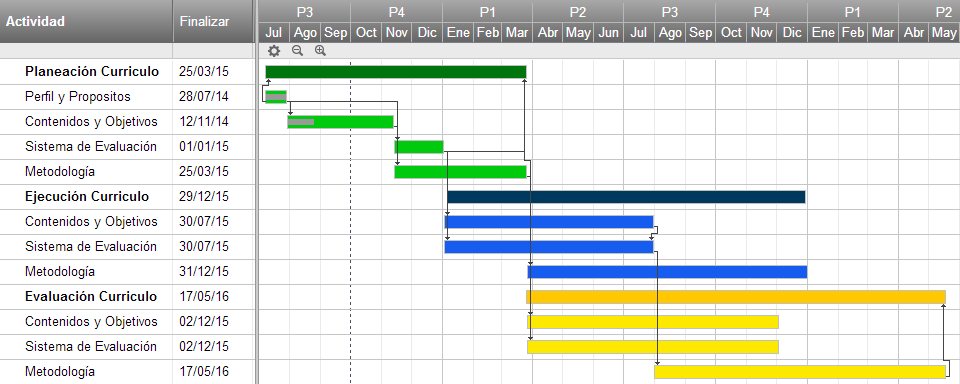
\includegraphics[scale=0.4]{gannt.png}
\end{figure}
\end{center}
\end{frame}
\section{Docentes}
\subsection{Planeaci\'on}
\subsection{Ejecuci\'on}
\subsection{Evaluaci\'on}
\section{Recursos}
\subsection{Planeaci\'on}
\subsection{Ejecuci\'on}
\subsection{Evaluaci\'on}
\section{Estudiantes}
\subsection{Planeac\'on}
\subsection{Ejecuci\'on}
\subsection{Evaluaci\'on}
\end{document}
